\documentclass[aspectratio=169,11pt]{beamer}
\usepackage[T1]{fontenc}
\usepackage{lmodern,amsmath,amssymb,mathtools,bm,booktabs,array,graphicx,tikz}
\usetikzlibrary{arrows.meta,positioning,calc,decorations.pathreplacing,patterns}
\definecolor{ink}{HTML}{17344D}\definecolor{accent}{HTML}{087E8B}\definecolor{pale}{HTML}{EDF5F5}\definecolor{gold}{HTML}{AD6B19}
\providecommand{\dd}{\,\mathrm{d}}\providecommand{\R}{\mathbb{R}}
\providecommand{\E}{\mathbb{E}}\providecommand{\Var}{\operatorname{Var}}
\providecommand{\Cov}{\operatorname{Cov}}\providecommand{\diag}{\operatorname{diag}}
\providecommand{\norm}[1]{\left\lVert#1\right\rVert}
\providecommand{\abs}[1]{\left|#1\right|}
\usefonttheme{professionalfonts}
\setbeamercolor{normal text}{fg=black,bg=white}
\setbeamercolor{frametitle}{fg=ink,bg=white}
\setbeamercolor{title}{fg=ink}\setbeamercolor{structure}{fg=accent}
\setbeamercolor{block title}{fg=ink,bg=pale}\setbeamercolor{block body}{fg=black,bg=pale!40}
\setbeamercolor{alerted text}{fg=accent}
\setbeamerfont{frametitle}{size=\Large,series=\bfseries}
\setbeamerfont{title}{size=\LARGE,series=\bfseries}
\setbeamertemplate{navigation symbols}{}
\setbeamersize{text margin left=.7cm,text margin right=.7cm}
\setbeamertemplate{frametitle}{\vspace{.18cm}\insertframetitle\par\vspace{.1cm}{\color{accent}\hrule height .6pt}\vspace{.12cm}}
\newcommand{\notestarget}{notes.pdf}\newcommand{\noteslabel}{Notes}
\setbeamertemplate{footline}{\hspace{.7cm}\color{ink}\scriptsize Scientific Computing in Python / 2027\quad\href{\notestarget}{\noteslabel}\hfill\insertframenumber\,/\,\inserttotalframenumber\hspace{.7cm}\vspace{.18cm}}
\setbeamercovered{invisible}
\hypersetup{pdfauthor={Zan Ahmad},pdftitle={Embeddings and scaled dot-product attention},pdfpagemode=UseNone}
\begin{document}
\begin{frame}[plain]\vfill
{\small\color{accent} Scientific Computing in Python / 2027 \quad Lecture 6}\par\medskip
{\raggedright\hyphenpenalty=10000\exhyphenpenalty=10000\LARGE\bfseries\color{ink} Embeddings and scaled dot-product attention}\par\bigskip
Zan Ahmad\par\smallskip
{\small Proposed 2027; calendar dates pending}\par\vfill\end{frame}
\renewcommand{\notestarget}{notes.pdf\#note-embedding-and-projection-matrices}
\begin{frame}[t,fragile,label=slide-embedding-and-projection-matrices]{Embedding and projection matrices}
\[
Q=XW_Q\in\R^{n\times d_k},\quad
K=XW_K\in\R^{n\times d_k},\quad
V=XW_V\in\R^{n\times d_v}.
\]
\pause{}
The score matrix $QK^{\mathsf T}$ has shape $n\times n$.
\end{frame}
\renewcommand{\notestarget}{notes.pdf\#note-embedding-and-projection-matrices}
\begin{frame}[t,fragile,label=slide-row-and-column-meanings]{Row and column meanings}
\[
S_{ij}=\frac{q_i^{\mathsf T}k_j}{\sqrt{d_k}}.
\]
\pause{}
Row $i$ fixes the query. Column $j$ identifies a key whose associated value may contribute to that query's output.
\end{frame}
\renewcommand{\notestarget}{notes.pdf\#note-rowwise-softmax}
\begin{frame}[t,fragile,label=slide-rowwise-softmax]{Rowwise softmax}
\[
A_{ij}=\frac{e^{S_{ij}}}{\sum_{\ell}e^{S_{i\ell}}},\qquad
A_{ij}>0,\quad\sum_jA_{ij}=1.
\]
\pause{}
Normalization is performed independently for each row.
\end{frame}
\renewcommand{\notestarget}{notes.pdf\#note-rowwise-softmax}
\begin{frame}[t,fragile,label=slide-stable-normalization]{Stable normalization}
For any row constant $c$,
\[
\frac{e^{s_j-c}}{\sum_\ell e^{s_\ell-c}}
=\frac{e^{s_j}}{\sum_\ell e^{s_\ell}}.
\]
\pause{}
Choose $c=\max_j s_j$ to avoid exponentiating large positive numbers.
\end{frame}
\renewcommand{\notestarget}{notes.pdf\#note-weighted-values}
\begin{frame}[t,fragile,label=slide-weighted-values]{Weighted values}
\[
Z=AV,\qquad z_i=\sum_j A_{ij}v_j.
\]
\pause{}
If every value is the same vector $v_*$, then $z_i=v_*$ for every row.
\end{frame}
\renewcommand{\notestarget}{notes.pdf\#note-rowwise-softmax}
\begin{frame}[label=slide-attention-weights-figure]{Attention weights}
\centering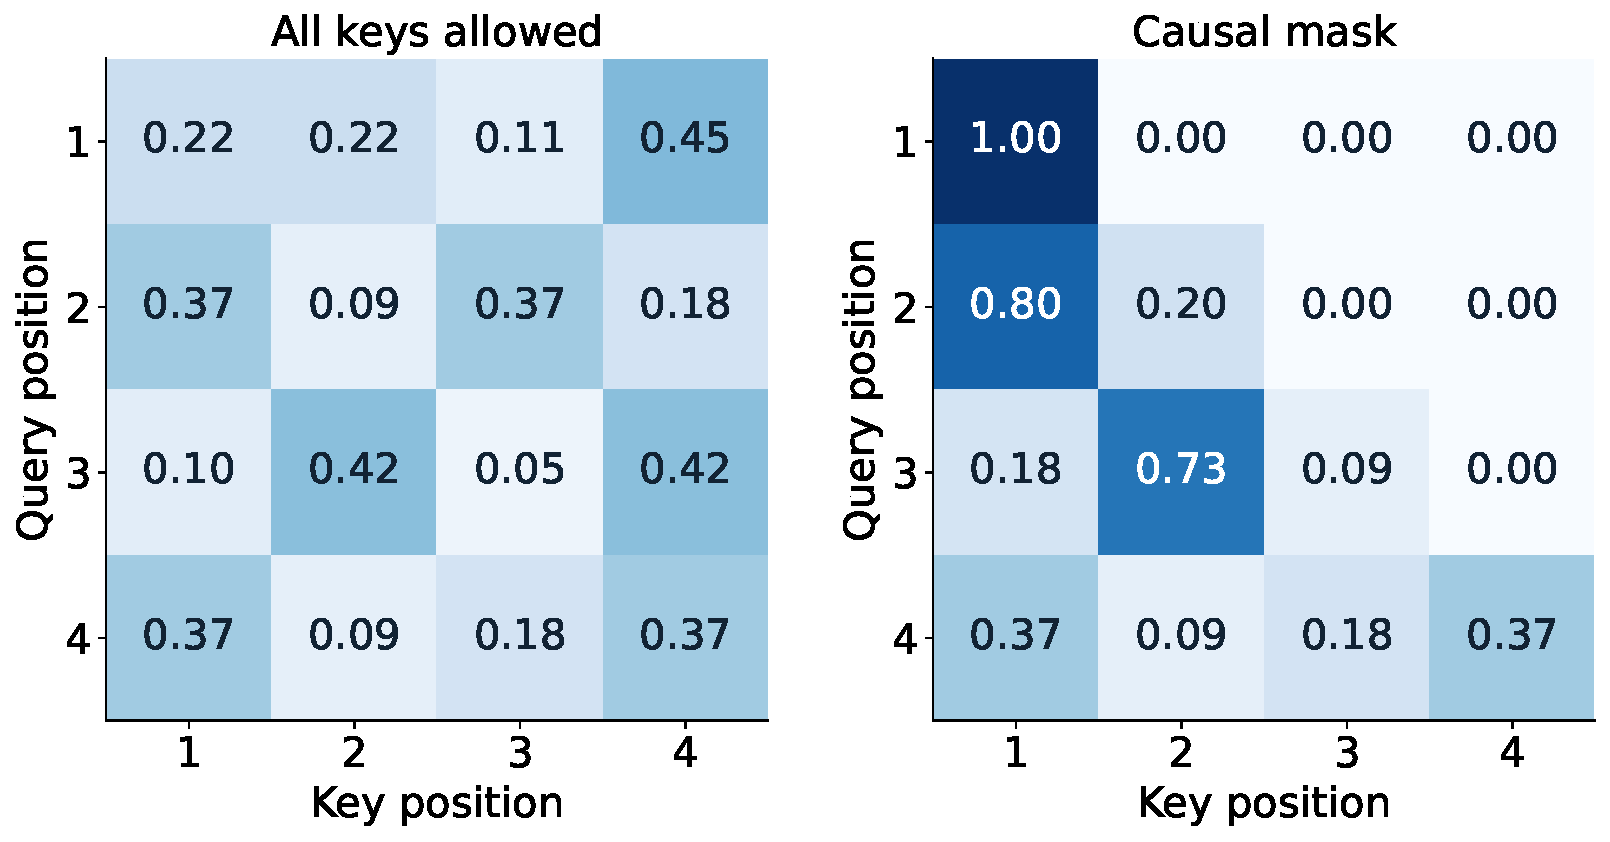
\includegraphics[width=.98\linewidth,height=.69\textheight,keepaspectratio]{attention-weights.pdf}\end{frame}
\renewcommand{\notestarget}{notes.pdf\#note-weighted-values}
\begin{frame}[t,fragile,label=slide-scaling-the-values]{Scaling the values}
With $Q$, $K$ and the allowed-key set fixed,
\[
A(\alpha V+\beta W)=\alpha AV+\beta AW.
\]
\pause{}
Doubling $V$ doubles $Z$. Changing $Q$ generally changes the weights themselves.
\end{frame}
\renewcommand{\notestarget}{notes.pdf\#note-a-two-key-calculation}
\begin{frame}[t,fragile,label=slide-a-two-key-calculation]{A two-key calculation}
\[
s=(1/\sqrt2,0),\qquad
A=\left(\frac{e^{1/\sqrt2}}{e^{1/\sqrt2}+1},\frac1{e^{1/\sqrt2}+1}\right).
\]
\pause{}
\[
A\approx(0.66976,0.33024).
\]
\end{frame}
\renewcommand{\notestarget}{notes.pdf\#note-a-two-key-calculation}
\begin{frame}[t,fragile,label=slide-the-output-vector]{The output vector}
\[
z=0.66976(2,0)+0.33024(0,4)
\approx(1.33952,1.32096).
\]
\pause{}
The two output coordinates are value coordinates. They need not sum to one and are not token probabilities.
\end{frame}
\renewcommand{\notestarget}{notes.pdf\#note-causal-masking}
\begin{frame}[t,fragile,label=slide-causal-masking]{Causal masking}
\[
A_{ij}=0\quad(j>i),\qquad
\sum_{j\leq i}A_{ij}=1.
\]
\pause{}
The first position has only one allowed key, hence $A_{11}=1$.
\end{frame}
\renewcommand{\notestarget}{notes.pdf\#note-causal-masking}
\begin{frame}[label=slide-weighted-values-2-figure]{Weighted values}
\centering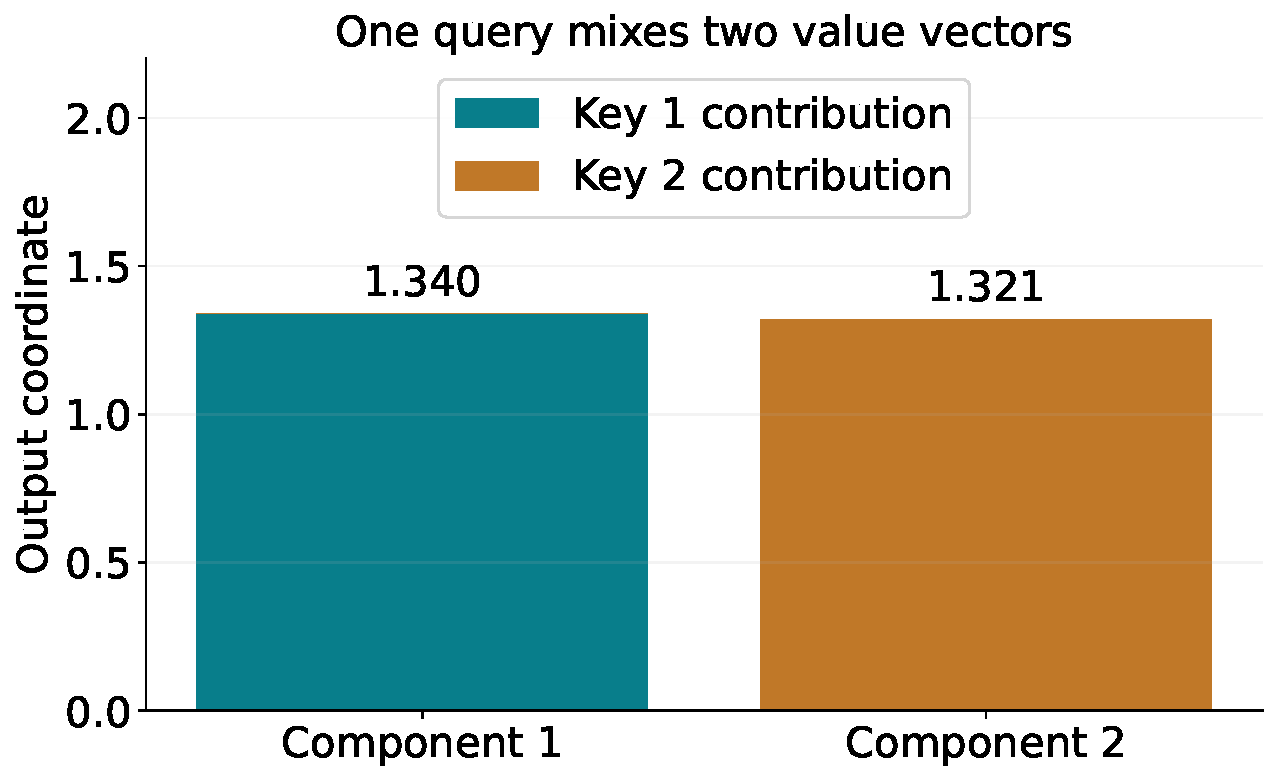
\includegraphics[width=.98\linewidth,height=.69\textheight,keepaspectratio]{weighted-values.pdf}\end{frame}
\renewcommand{\notestarget}{notes.pdf\#note-causal-masking}
\begin{frame}[t,fragile,label=slide-a-causal-perturbation-test]{A causal perturbation test}
Change only the final embedding row while holding projection matrices fixed.
\pause{}
Earlier causal outputs remain unchanged. Earlier unmasked outputs can change because the final key and value are available to them.
\end{frame}
\renewcommand{\notestarget}{notes.pdf\#note-scaling-and-learned-representations}
\begin{frame}[t,fragile,label=slide-scaling-and-learned-representations]{Scaling and learned representations}
Under independent, zero-mean, unit-variance coordinates,
\[
\operatorname{Var}\left(\sum_{r=1}^{d_k}q_rk_r\right)=d_k.
\]
\pause{}
Dividing by $\sqrt{d_k}$ keeps the variance at one.
\end{frame}
\renewcommand{\notestarget}{notes.pdf\#note-scaling-and-learned-representations}
\begin{frame}[t,fragile,label=slide-permutation-and-position]{Permutation and position}
Without positional information, permuting input rows by $P$ gives
\[
Q'=PQ,\ K'=PK,\ V'=PV\quad\Longrightarrow\quad Z'=PZ
\]
for unmasked attention.
\pause{}
Position encodings or structured masks provide information not present in an unordered collection of embedding rows.
\end{frame}
\end{document}
